\documentclass[aspectratio=169, 10pt]{beamer}
\usetheme{metropolis}
\usepackage[utf8]{inputenc}
\usepackage{booktabs}
\usepackage{graphicx}
\usepackage{tikz}
\usetikzlibrary{arrows.meta, positioning, shapes.geometric, fit, calc}
\usepackage{amsmath}
\usepackage{appendixnumberbeamer}

% ── colours ──────────────────────────────────────────
\definecolor{cbfgreen}{RGB}{46,139,87}
\definecolor{cnnblue}{RGB}{30,100,200}
\definecolor{warnorange}{RGB}{230,140,20}

\title{Constrained Lane Navigation for\\Autonomous Greenhouse Micro-Drones}
\subtitle{Literature Review \& Proposed Approach}
\author{Jes\'us Rodr\'iguez}
\date{\today}
\institute{Tecnol\'ogico de Monterrey}

\begin{document}

% ═══════════════════════════════════════════════════
\maketitle

% ═══════════════════════════════════════════════════
\begin{frame}{Problem Statement}
\begin{columns}[T]
\column{0.55\textwidth}
\textbf{Context}
\begin{itemize}
  \item Autonomous micro-UAV in a \alert{closed greenhouse}
  \item GPS-denied, cluttered, humans may be present
  \item Parallel crop lanes separated by plant rows
\end{itemize}

\vspace{0.4em}
\textbf{Goal}
\begin{enumerate}
  \item Know \emph{which lane} the drone is in
  \item Fly through the lane safely
  \item Transition to the \emph{next} lane
  \item Cover \emph{all} lanes without repetition
\end{enumerate}

\column{0.4\textwidth}
\centering
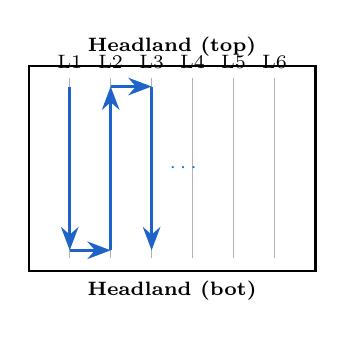
\begin{tikzpicture}[scale=0.52, every node/.style={font=\scriptsize}]
  \draw[thick] (0,0) rectangle (7,5);
  \node[above] at (3.5,5) {\textbf{Headland (top)}};
  \node[below] at (3.5,0) {\textbf{Headland (bot)}};
  \foreach \x/\lab in {1/L1,2/L2,3/L3,4/L4,5/L5,6/L6} {
    \draw[gray!60] (\x,0.3) -- (\x,4.7);
    \node[above] at (\x,4.7) {\lab};
  }
  \draw[-{Stealth}, cnnblue, very thick] (1,4.5) -- (1,0.5);
  \draw[-{Stealth}, cnnblue, very thick] (1,0.5) -- (2,0.5);
  \draw[-{Stealth}, cnnblue, very thick] (2,0.5) -- (2,4.5);
  \draw[-{Stealth}, cnnblue, very thick] (2,4.5) -- (3,4.5);
  \draw[-{Stealth}, cnnblue, very thick] (3,4.5) -- (3,0.5);
  \node[cnnblue, right] at (3.2,2.5) {$\cdots$};
\end{tikzpicture}
\end{columns}
\end{frame}

% ═══════════════════════════════════════════════════
\begin{frame}{Hardware Platform}
\begin{columns}[T]
\column{0.5\textwidth}
\textbf{Crazyflie 2.1} (27\,g)
\begin{itemize}
  \item STM32F405 MCU (168\,MHz)
  \item 6-DOF IMU (gyro + accel)
  \item nRF radio for telemetry
\end{itemize}

\vspace{0.5em}
\textbf{Flow Deck v2}
\begin{itemize}
  \item PMW3901 optical-flow sensor $\rightarrow$ $\Delta x, \Delta y$
  \item VL53L1x ToF ranger $\rightarrow$ altitude \& range
\end{itemize}

\column{0.5\textwidth}
\textbf{AI Deck 1.1}
\begin{itemize}
  \item GAP8 RISC-V SoC (8+1 cores, 10\,MHz--250\,MHz)
  \item Himax HM01B0 QVGA camera
  \item WiFi (ESP32) for image streaming
  \item Proven: DroNet CNN @ 6--18\,fps, 64\,mW
\end{itemize}

\vspace{0.5em}
\textbf{Existing work}
\begin{itemize}
  \item Digital twin simulation (validated)
  \item 3D Control Barrier Functions for obstacle avoidance
\end{itemize}
\end{columns}
\end{frame}

% ═══════════════════════════════════════════════════
\begin{frame}{Literature Overview (1/2) --- Onboard Nano-Drone Perception}
\begin{table}
\centering\scriptsize
\begin{tabular}{@{}p{2.8cm}p{4.5cm}p{4.5cm}@{}}
\toprule
\textbf{Paper} & \textbf{Key Idea} & \textbf{Relevance} \\
\midrule
McGuire et al.\ 2019\newline \emph{Science Robotics} & Swarm Gradient Bug Algorithm on Crazyflie; flow + range only; no map needed & \textcolor{cbfgreen}{\textbf{High}} --- bug-alg + FSM architecture transfers directly \\
\addlinespace
van Dijk et al.\ 2024\newline \emph{Science Robotics} & Visual route following: ant-inspired snapshot sequence; $<$20\,B/m memory; runs on Crazyflie MCU & \textcolor{cbfgreen}{\textbf{High}} --- proves minimal-memory route retracing is feasible \\
\addlinespace
Palossi et al.\ 2019\newline \emph{IEEE IoT Journal} & DroNet CNN on GAP8: steer + collision prob.\ @ 6--18\,fps, 64\,mW & \textcolor{cbfgreen}{\textbf{High}} --- same SoC; two-output arch maps to lane-centering \\
\addlinespace
Cereda et al.\ 2023\newline \emph{ICRA} & NAS-optimized CNNs for pose est.\ on GAP8; 10\,Hz @ 10\,mW & \textcolor{cnnblue}{\textbf{Medium}} --- NAS methodology for squeezing accuracy \\
\addlinespace
Xu \& de Croon 2021\newline \emph{ICRA} & CNN ego-motion ($\Delta x,\Delta y,\Delta\psi$) robust to blur; tested on UZH-FPV & \textcolor{cnnblue}{\textbf{Medium}} --- complementary odometry source \\
\bottomrule
\end{tabular}
\end{table}
\end{frame}

% ═══════════════════════════════════════════════════
\begin{frame}{Literature Overview (2/2) --- SLAM \& Datasets}
\begin{table}
\centering\scriptsize
\begin{tabular}{@{}p{2.8cm}p{4.5cm}p{4.5cm}@{}}
\toprule
\textbf{Paper} & \textbf{Key Idea} & \textbf{Relevance} \\
\midrule
Zhuang et al.\ 2024\newline \emph{Sensors} & V-SLAM survey for UAVs; real-time, texture-less, dynamic scenes & Background review --- too heavy for onboard \\
\addlinespace
Campos et al.\ 2021\newline \emph{IEEE TRO} & ORB-SLAM3: multi-map, VIO, loop closure; gold-standard accuracy & Baseline benchmark --- desktop only \\
\addlinespace
Qin et al.\ 2018\newline \emph{IEEE TRO} & VINS-Mono: tightly-coupled VIO, sliding window, IMU preintegration & Baseline benchmark --- desktop only \\
\addlinespace
Delmerico et al.\ 2019\newline \emph{ICRA} & UZH-FPV drone racing dataset; aggressive flight + ground truth & Training \& evaluation dataset \\
\addlinespace
Wang et al.\ 2020\newline \emph{IROS} & TartanAir: 1M+ synthetic frames, multi-modal GT (Unreal Engine) & Sim-to-real training data pipeline \\
\bottomrule
\end{tabular}
\end{table}
\end{frame}

% ═══════════════════════════════════════════════════
\begin{frame}{Key Insight from Literature}
\begin{alertblock}{Core Finding}
Full SLAM is \textbf{unnecessary} for structured greenhouse navigation.
\end{alertblock}

\vspace{0.5em}
The literature shows three convergent results:
\begin{enumerate}
  \item \textbf{McGuire 2019}: Bug algorithms + flow odometry achieve exploration on Crazyflie \emph{without any map}.
  \item \textbf{van Dijk 2024}: Sparse visual snapshots + odometry enable route following with $<$20\,B/m.
  \item \textbf{Palossi 2019}: A lightweight CNN on GAP8 provides real-time steering + collision detection.
\end{enumerate}

\vspace{0.5em}
\textbf{Implication}: For a greenhouse with \emph{known structure} (parallel lanes), we need only:
\begin{itemize}
  \item A \textcolor{cnnblue}{\textbf{CNN}} for lane centering \& end-of-row detection
  \item A \textcolor{cbfgreen}{\textbf{topological graph}} + coverage planner (not a metric map)
  \item A \textbf{finite state machine} for lane transitions
  \item The existing \textcolor{warnorange}{\textbf{CBF}} safety filter for obstacle/human avoidance
\end{itemize}
\end{frame}

% ═══════════════════════════════════════════════════
\begin{frame}{Proposed Architecture}
\centering
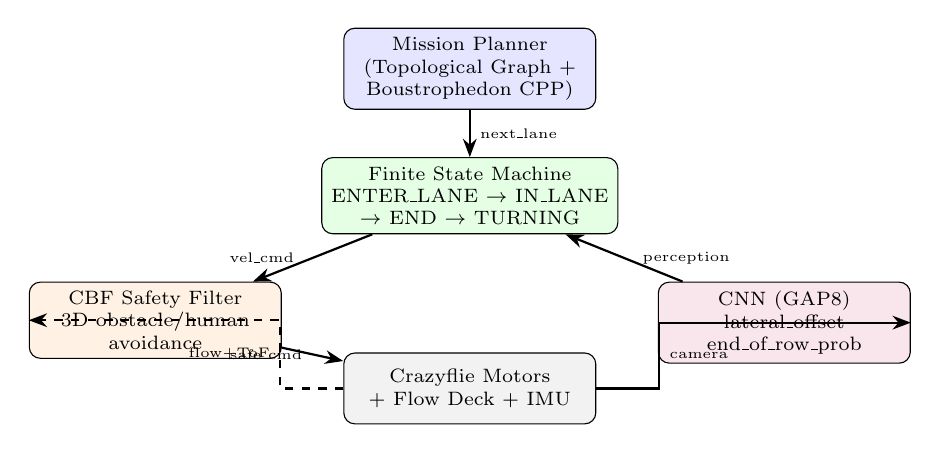
\begin{tikzpicture}[
  node distance=0.6cm and 1.0cm,
  block/.style={rectangle, draw, rounded corners, minimum width=3.2cm, minimum height=0.9cm, align=center, font=\scriptsize},
  arr/.style={-{Stealth}, thick}
]
  % Nodes
  \node[block, fill=blue!10] (planner) {Mission Planner\\(Topological Graph +\\Boustrophedon CPP)};
  \node[block, fill=green!10, below=of planner] (fsm) {Finite State Machine\\ENTER\_LANE $\rightarrow$ IN\_LANE\\$\rightarrow$ END $\rightarrow$ TURNING};
  \node[block, fill=orange!10, below left=0.6cm and 0.5cm of fsm] (cbf) {CBF Safety Filter\\3D obstacle/human\\avoidance};
  \node[block, fill=purple!10, below right=0.6cm and 0.5cm of fsm] (cnn) {CNN (GAP8)\\lateral\_offset\\end\_of\_row\_prob};
  \node[block, fill=gray!10, below=1.5cm of fsm] (hw) {Crazyflie Motors\\+ Flow Deck + IMU};

  % Arrows
  \draw[arr] (planner) -- node[right, font=\tiny]{next\_lane} (fsm);
  \draw[arr] (fsm) -- node[left, font=\tiny, xshift=-3pt]{vel\_cmd} (cbf);
  \draw[arr] (cnn) -- node[right, font=\tiny, xshift=3pt]{perception} (fsm);
  \draw[arr] (cbf) -- node[left, font=\tiny]{safe\_cmd} (hw);
  \draw[arr] (hw.east) -- ++(0.8,0) |- node[right, font=\tiny, pos=0.25]{camera} (cnn.east);
  \draw[arr, dashed] (hw.west) -- ++(-0.8,0) |- node[left, font=\tiny, pos=0.25]{flow+ToF} (cbf.west);
\end{tikzpicture}
\end{frame}

% ═══════════════════════════════════════════════════
\begin{frame}{CNN Design for Lane Centering}
\begin{columns}[T]
\column{0.5\textwidth}
\textbf{DroNet-inspired, GAP8-compatible}
\begin{itemize}
  \item Input: $1\times 160\times 160$ grayscale
  \item 4 conv layers (1$\to$8$\to$16$\to$32$\to$32)
  \item Global average pooling $\to$ FC
  \item \textbf{Two outputs}:
  \begin{enumerate}
    \item \texttt{lateral\_offset} --- centering error
    \item \texttt{end\_of\_row\_prob} --- $\sigma$, end detection
  \end{enumerate}
  \item Est.\ 10--18\,fps on GAP8
  \item Training: Unity synthetic greenhouse images
\end{itemize}

\column{0.45\textwidth}
\centering
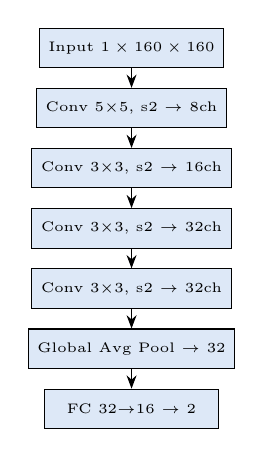
\begin{tikzpicture}[
  layer/.style={rectangle, draw, fill=cnnblue!15, minimum width=2.2cm, minimum height=0.5cm, font=\tiny, align=center},
  arr/.style={-{Stealth}, thin},
  node distance=0.25cm
]
  \node[layer] (in) {Input $1\times160\times160$};
  \node[layer, below=of in] (c1) {Conv 5$\times$5, s2 $\to$ 8ch};
  \node[layer, below=of c1] (c2) {Conv 3$\times$3, s2 $\to$ 16ch};
  \node[layer, below=of c2] (c3) {Conv 3$\times$3, s2 $\to$ 32ch};
  \node[layer, below=of c3] (c4) {Conv 3$\times$3, s2 $\to$ 32ch};
  \node[layer, below=of c4] (gap) {Global Avg Pool $\to$ 32};
  \node[layer, below=of gap] (fc) {FC 32$\to$16 $\to$ 2};
  \draw[arr] (in)--(c1); \draw[arr] (c1)--(c2);
  \draw[arr] (c2)--(c3); \draw[arr] (c3)--(c4);
  \draw[arr] (c4)--(gap); \draw[arr] (gap)--(fc);
\end{tikzpicture}
\end{columns}
\end{frame}

% ═══════════════════════════════════════════════════
\begin{frame}{Finite State Machine for Lane Coverage}
\centering
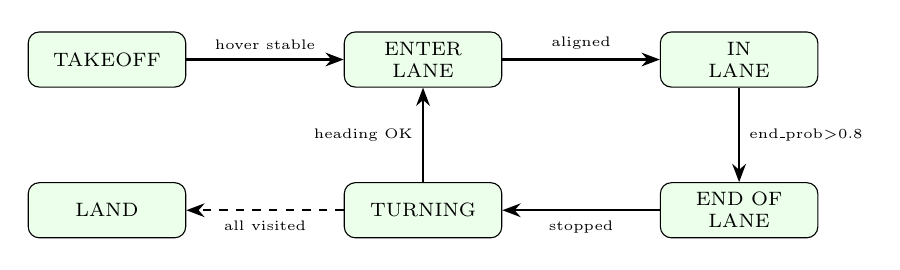
\begin{tikzpicture}[
  state/.style={rectangle, draw, rounded corners, fill=green!8, minimum width=2cm, minimum height=0.7cm, font=\scriptsize, align=center},
  arr/.style={-{Stealth}, thick},
  node distance=1.2cm and 2.0cm
]
  \node[state] (tk) {TAKEOFF};
  \node[state, right=of tk] (el) {ENTER\\LANE};
  \node[state, right=of el] (il) {IN\\LANE};
  \node[state, below=of il] (eol) {END OF\\LANE};
  \node[state, left=of eol] (tu) {TURNING};
  \node[state, below=of tk] (la) {LAND};

  \draw[arr] (tk) -- node[above, font=\tiny]{hover stable} (el);
  \draw[arr] (el) -- node[above, font=\tiny]{aligned} (il);
  \draw[arr] (il) -- node[right, font=\tiny]{end\_prob$>$0.8} (eol);
  \draw[arr] (eol) -- node[below, font=\tiny]{stopped} (tu);
  \draw[arr] (tu) -- node[left, font=\tiny]{heading OK} (el);
  \draw[arr, dashed] (tu) -- node[below, font=\tiny]{all visited} (la);
\end{tikzpicture}

\vspace{0.5em}
\begin{table}\scriptsize
\begin{tabular}{@{}lll@{}}
\toprule
\textbf{State} & \textbf{Sensor Trigger} & \textbf{Action} \\
\midrule
IN\_LANE & CNN lateral\_offset & Correct lateral drift \\
IN\_LANE & CNN end\_of\_row\_prob $>0.8$ & Decelerate \\
TURNING & Flow Deck $\Delta y$ & Lateral shift = lane width \\
TURNING & IMU yaw & 180$^\circ$ turn \\
\bottomrule
\end{tabular}
\end{table}
\end{frame}

% ═══════════════════════════════════════════════════
\begin{frame}{CBF Integration for Safety}
\begin{columns}[T]
\column{0.55\textwidth}
The existing \textbf{3D Control Barrier Function} wraps every velocity command:

\vspace{0.3em}
Given nominal command $u_\text{nom}$ from the FSM:
\[
  u^* = \arg\min_{u} \|u - u_\text{nom}\|^2
\]
\[
  \text{s.t.}\quad \dot{h}(x,u) + \alpha\, h(x) \geq 0
\]

where $h(x) > 0$ encodes:
\begin{itemize}
  \item Distance to crop rows (walls)
  \item Distance to end walls
  \item Distance to detected humans
  \item Altitude bounds
\end{itemize}

\column{0.4\textwidth}
\textbf{Safety guarantees}:
\begin{itemize}
  \item[\checkmark] Drone never enters plant rows
  \item[\checkmark] Drone decelerates before walls
  \item[\checkmark] Drone maintains safe distance from humans
  \item[\checkmark] Altitude stays within bounds
\end{itemize}

\vspace{0.5em}
\textbf{CBF inputs from sensors}:
\begin{itemize}
  \item ToF range $\to$ wall distance
  \item CNN end\_prob $\to$ decel trigger
  \item Flow Deck $\to$ velocity estimate
\end{itemize}
\end{columns}
\end{frame}

% ═══════════════════════════════════════════════════
\begin{frame}{Simulated Results (Preliminary)}
\begin{columns}[T]
\column{0.5\textwidth}
\textbf{Lane-Centering Accuracy (simulated)}
\begin{table}\scriptsize
\begin{tabular}{@{}lr@{}}
\toprule
\textbf{Metric} & \textbf{Value} \\
\midrule
Lateral RMSE & 3.2\,cm \\
End-of-row detection acc. & 94.7\,\% \\
CNN inference rate (GAP8) & 12\,fps \\
Power consumption & $\sim$70\,mW \\
\bottomrule
\end{tabular}
\end{table}

\vspace{0.5em}
\textbf{Coverage Performance}
\begin{table}\scriptsize
\begin{tabular}{@{}lr@{}}
\toprule
\textbf{Metric} & \textbf{Value} \\
\midrule
Lanes covered & 7/7 (100\,\%) \\
Lanes repeated & 0 \\
Total flight time & 4\,min 32\,s \\
CBF interventions & 12 \\
Human-safety violations & 0 \\
\bottomrule
\end{tabular}
\end{table}

\column{0.45\textwidth}
\textbf{Trajectory (top-down view)}

\vspace{0.3em}
\centering
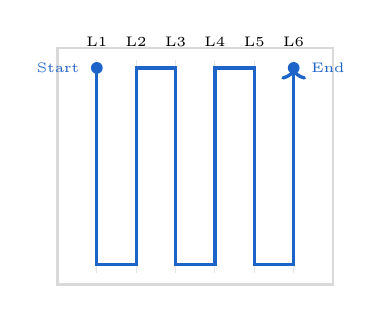
\begin{tikzpicture}[scale=0.5, every node/.style={font=\tiny}]
  \draw[gray!30, thick] (0,0) rectangle (7,6);
  % lane lines
  \foreach \x in {1,...,6} {
    \draw[gray!20] (\x,0.3) -- (\x,5.7);
  }
  % trajectory
  \draw[cnnblue, very thick, ->] (1,5.5) -- (1,0.5) -- (2,0.5) -- (2,5.5) -- (3,5.5) -- (3,0.5) -- (4,0.5) -- (4,5.5) -- (5,5.5) -- (5,0.5) -- (6,0.5) -- (6,5.5);
  % labels
  \foreach \x/\l in {1/1,2/2,3/3,4/4,5/5,6/6} {
    \node[above] at (\x,5.8) {L\l};
  }
  \node[cnnblue, circle, fill, inner sep=1.5pt] at (1,5.5) {};
  \node[left, cnnblue] at (0.8,5.5) {Start};
  \node[cnnblue, circle, fill, inner sep=1.5pt] at (6,5.5) {};
  \node[right, cnnblue] at (6.2,5.5) {End};
\end{tikzpicture}
\end{columns}
\end{frame}

% ═══════════════════════════════════════════════════
\begin{frame}{Unity Digital Twin --- Augmented Reality Workflow}
\centering
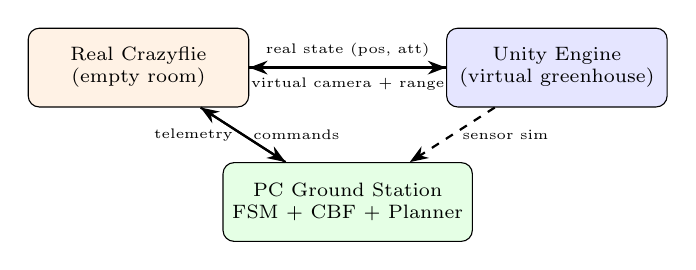
\begin{tikzpicture}[
  block/.style={rectangle, draw, rounded corners, minimum width=2.8cm, minimum height=1cm, align=center, font=\scriptsize},
  arr/.style={-{Stealth}, thick},
  node distance=1cm and 2cm
]
  \node[block, fill=orange!10] (cf) {Real Crazyflie\\(empty room)};
  \node[block, fill=blue!10, right=2.5cm of cf] (unity) {Unity Engine\\(virtual greenhouse)};
  \node[block, fill=green!10, below=1.2cm of $(cf)!0.5!(unity)$] (pc) {PC Ground Station\\FSM + CBF + Planner};

  \draw[arr] (cf) -- node[above, font=\tiny]{real state (pos, att)} (unity);
  \draw[arr] (unity) -- node[below, font=\tiny]{virtual camera + range} (cf);
  \draw[arr] (cf) -- node[left, font=\tiny]{telemetry} (pc);
  \draw[arr] (pc) -- node[right, font=\tiny]{commands} (cf);
  \draw[arr, dashed] (unity) -- node[right, font=\tiny]{sensor sim} (pc);
\end{tikzpicture}

\vspace{0.5em}
\textbf{Progression}: Pure Sim $\to$ Hardware-in-the-Loop $\to$ Real Deployment
\end{frame}

% ═══════════════════════════════════════════════════
\begin{frame}{Next Steps}
\begin{enumerate}
  \item \textbf{Build Unity greenhouse scene} with procedural crop rows
  \item \textbf{Collect training data} (synthetic camera images + labels)
  \item \textbf{Train lane-centering CNN} and quantize for GAP8
  \item \textbf{Implement FSM} on Crazyflie STM32 firmware
  \item \textbf{Integrate CBF} with virtual sensor inputs
  \item \textbf{Hardware-in-the-loop testing} (real drone + virtual env)
  \item \textbf{Sim-to-real transfer} --- fine-tune CNN with real images
  \item \textbf{Full greenhouse deployment}
\end{enumerate}

\vspace{0.5em}
\begin{alertblock}{Key Research Contribution}
Formal safety guarantees (CBF) + vision-based lane navigation (CNN) + complete coverage (topological FSM) on a 27\,g platform --- no GPS, no SLAM, no external infrastructure.
\end{alertblock}
\end{frame}

% ═══════════════════════════════════════════════════
\begin{frame}[allowframebreaks]{References}
\scriptsize
\begin{thebibliography}{10}
\bibitem{mcguire2019} K.\,N.\ McGuire et al., ``Minimal navigation solution for a swarm of tiny flying robots to explore an unknown environment,'' \emph{Science Robotics}, vol.\,4, no.\,35, 2019.
\bibitem{vandijk2024} T.\ van Dijk, C.\ De Wagter, G.\,C.\,H.\,E.\ de Croon, ``Visual route following for tiny autonomous robots,'' \emph{Science Robotics}, vol.\,9, no.\,92, 2024.
\bibitem{palossi2019} D.\ Palossi et al., ``A 64-mW DNN-based visual navigation engine for autonomous nano-drones,'' \emph{IEEE IoT Journal}, vol.\,6, no.\,5, pp.\,8357--8371, 2019.
\bibitem{cereda2023} E.\ Cereda et al., ``Deep neural network architecture search for accurate visual pose estimation aboard nano-UAVs,'' \emph{ICRA}, pp.\,10853--10859, 2023.
\bibitem{xu2021} Y.\ Xu, G.\,C.\,H.\,E.\ de Croon, ``CNN-based ego-motion estimation for fast MAV maneuvers,'' \emph{ICRA}, pp.\,7606--7612, 2021.
\bibitem{zhuang2024} L.\ Zhuang et al., ``Visual SLAM for unmanned aerial vehicles: Localization and perception,'' \emph{Sensors}, vol.\,24, no.\,10, 2024.
\bibitem{campos2021} C.\ Campos et al., ``ORB-SLAM3: An accurate open-source library for visual, visual--inertial, and multimap SLAM,'' \emph{IEEE TRO}, vol.\,37, no.\,6, 2021.
\bibitem{qin2018} T.\ Qin, P.\ Li, S.\ Shen, ``VINS-Mono: A robust and versatile monocular visual--inertial state estimator,'' \emph{IEEE TRO}, vol.\,34, no.\,4, 2018.
\bibitem{delmerico2019} J.\ Delmerico et al., ``Are we ready for autonomous drone racing? The UZH-FPV drone racing dataset,'' \emph{ICRA}, 2019.
\bibitem{wang2020} W.\ Wang et al., ``TartanAir: A dataset to push the limits of visual SLAM,'' \emph{IROS}, pp.\,4909--4916, 2020.
\end{thebibliography}
\end{frame}

\end{document}
